\documentclass[12pt]{article}
\newcommand{\VERSION}{0.0-2}
%\VignetteIndexEntry{addingToolkit}
%\VignettePackage{addingToolkit}

\usepackage{times}              % for fonts
\usepackage[]{geometry}
\usepackage{mathptm}            % for math fonts type 1
\usepackage{graphicx}           % for graphics files
\usepackage{floatflt}           % for ``floating boxes''
%%\usepackage{index}
\usepackage{relsize}            % for relative size fonts
\usepackage{amsmath}            % for amslatex stuff
\usepackage{amsfonts}           % for amsfonts
\usepackage{url}                % for \url,
\usepackage{color}
\usepackage{fancyvrb}
\usepackage{fancyhdr}
%%\usepackage{jvfloatstyle}       % redefine float.sty for my style. Hack


%% squeeze in stuff
%%\floatstyle{jvstyle}
%%\restylefloat{table}
%%\restylefloat{figure}
\renewcommand\floatpagefraction{.9}
\renewcommand\topfraction{.9}
\renewcommand\bottomfraction{.9}
\renewcommand\textfraction{.1}
\setcounter{totalnumber}{50}
\setcounter{topnumber}{50}
\setcounter{bottomnumber}{50}

%% Fill these in
\pagestyle{fancy}
\usepackage{fancyhdr}
\pagestyle{fancy}
\fancyhf{}
\fancyhead[L]{\RCode{gWidgets}}
\fancyhead[C]{}
\fancyhead[R]{\sectionmark}
\fancyfoot[L]{}
\fancyfoot[C]{- page \thepage\/ -}
\fancyfoot[R]{}
\renewcommand{\headrulewidth}{0.1pt}
\renewcommand{\footrulewidth}{0.0pt}

%% My abbreviations
\newcommand{\RCode}[1]{\texttt{#1}}
\newcommand{\RFunc}[1]{\texttt{#1()}}
\newcommand{\RPackage}[1]{\textbf{#1}}
\newcommand{\RArg}[1]{\texttt{#1=}}
\newcommand{\RListel}[1]{\texttt{\$#1}}


\newenvironment{RArgs}{\begin{list}{}{}}{\end{list}}


\usepackage{/home/verzani/R//lib/R/share/texmf/Sweave}
\begin{document}
\thispagestyle{plain}
\title{Adding a toolkit to gWidgets}

\author{John Verzani, \url{gWidgetsRGtk@gmail.com}}
\maketitle

\section*{Abstract:}
[\textbf{This package is now out of date. The \RPackage{gWidgetstcltk} package
has been written. This is here in case someone wants to port a
different toolkit (RwxWidgets say).}]
\\

This little vignette illustrates what is required to write a toolkit
for the \RPackage{gWidgets} package. Since the \RPackage{gWidgetsRGtk}
package is written this sketches out what a toolkit would possibly
look like using the \RPackage{tcltk} package.

\setcounter{tocdepth}{3}
\tableofcontents

\section{Basics of gWidgets}

The gWidgets implementation is simply a set of functions that dispatch
to similarly named functions in a toolkit. That is the
\RCode{glabel(...,toolkit=guiToolkit())} function dispatches to the
\RCode{.glabel(toolkit, ...)} function in the appropriate toolkit, and
the \RCode{svalue(obj,...)} method dispatches to the
\RCode{.svalue(obj@widget,obj@toolkit, ...)} function in the
appropriate toolkit. In the first case, a constructor, the dispatch is
done by the class of the toolkit. For the method, the dispatch is
based on both the toolkit and the class of the object, and perhaps
other arguments in the signature of the method.

The classes for the toolkits \RCode{RGtk2}, \RCode{tcltk}, \RCode{rJava}, and \RCode{SJava} are already defined by gWidgets. These are named \RCode{guiWidgetsToolkit} plus the package name.


As such, the basic structure of a gWidgets implementation is to set up
some classes, and a set of methods for dispatch.~\footnote{Although it
likely wasn't necessary, at the time of first writing a package, the
dispatch was to a "dot" file. This caused an extra level to the
dispatch, that while unfortunate, does not seem to be worth rewriting
to avoid.}


\section{An example}


This shows some of what is necessary to write an implementation of
gWidgets for the \RPackage{tcltk} package.  It only assumes as much
about \RPackage{tcltk} as was learned by browsing Peter Dalgaard's
informative RNews article and a quick glance at the examples provided
by James Wettenhall.




First we load the package.
\begin{Scode}
  ## load toolkit 
  options("guiToolkit"=NA)
  library(gWidgets)
  library(tcltk)
\end{Scode}

The options setting ensures no toolkit for gWidgets gets loaded.

We note the subclass of \RCode{guiWidgetsToolkit},
\RCode{guiWidgetsToolkittcltk} is already defined in \RCode{gWidgets}.

Now we make a base class for the tcltk widgets created here.
\begin{Scode}
  ## some classes
  setClass("gWidgetTcltk")
  ## A virtual class to hold tcltk object or guiWidget or gWidgetTcltk
  setClass("guiWidgetORgWidgetTcltkORtcltk")
  setIs("guiWidget","guiWidgetORgWidgetTcltkORtcltk")
  setIs("gWidgetTcltk","guiWidgetORgWidgetTcltkORtcltk")
\end{Scode}

Finally, we promote the \RCode{tkwin} class to an S4 class and add it
to our virtual class. This would be done for all possible classes of
\RCode{tcltk} objects.

\begin{Scode}
  oldclasses = c("tkwin")
  for(i in oldclasses) {
    setOldClass(i)
    setIs(i,"guiWidgetORgWidgetTcltkORtcltk")
  }
\end{Scode}


The \RCode{gWidgetTcltk} class is a virtual class, here are two
subclasses. We create slots for the widget and the toolkit here, but
perhaps should add others such as an ID slot for storing a unique ID
per widget.

\begin{Scode}
### Make some base classes
setClass("gComponentTcltk",
representation(
widget="guiWidgetORgWidgetTcltkORtcltk",
toolkit="guiWidgetsToolkit"
),
contains="gWidgetTcltk",
)
setClass("gContainerTcltk",
representation(
widget="guiWidgetORgWidgetTcltkORtcltk",
toolkit="guiWidgetsToolkit"
),
contains="gWidgetTcltk",
)
\end{Scode}

Now we define some necessary functions to implement \RFunc{gwindow} in
the toolkit. This involves defining a class, making a constructor
(\RFunc{.gwindow}) and defining some methods.

\begin{Scode}
## top level window
setClass("gWindowTcltk",
contains="gContainerTcltk",
prototype=prototype(new("gContainerTcltk"))
)
\end{Scode}

This implementation of the constructor should have a handler for the
window destroy event.
\begin{Scode}
  setMethod(".gwindow",
  signature(toolkit="guiWidgetsToolkittcltk"),
  function(toolkit,
  title="Window", visible=TRUE,
  handler=NULL, action = NULL,
  ...
  ) {
    win <- tktoplevel()
    tktitle(win) <- title
    
    obj = new("gWindowTcltk", widget=win, toolkit=toolkit)
    return(obj)
  })
\end{Scode}

The \RFunc{svalue} method for \RFunc{gwindow} objects is used to
retrieve and set the title of the window. 

\begin{Scode}
setMethod(".svalue",
signature(toolkit="guiWidgetsToolkittcltk",obj="gWindowTcltk"),
function(obj, toolkit, index=NULL, drop=NULL, ..) {
  tktitle(obj@widget)
})

setMethod(".svalue<-",
signature(toolkit="guiWidgetsToolkittcltk",obj="gWindowTcltk"),
function(obj, toolkit, index=NULL,..., value) {
  ## set the title
  tktitle(obj@widget) <- value
  return(obj)
})
\end{Scode}

The \RFunc{add} method is used to add a widget to a container. This is
where we run into problems with \RPackage{tcltk} as the constructors
there require a ``parent'' container at the time of construction. As
such, we don't have both a container (\RCode{obj} below) and  widget
(\RCode{value}) needed when we add, rather we only specify how things
are packed in.

\begin{Scode}
setMethod(".add",
signature(toolkit="guiWidgetsToolkittcltk",obj="gWindowTcltk",
value="guiWidget"),
function(obj, toolkit, value, ...) {
  ## how to add?
  tkpack(value@widget@widget)
})
\end{Scode}

[To avoid this, the \RPackage{gWidgetstcltk} package requires a
container be specified when a widget is constructed. This container
stores the top-level container so that a \RPackage{tcltk} widget can
be constructed. The \RCode{add} method is then rarely used publicly,
but is useful when writing the constructor. It's
arguments for placement of the widget are specified during the
construction of the widget.]

The \RCode{dispose} method closes the window
\begin{Scode}
setMethod(".dispose",
          signature(toolkit="guiWidgetsToolkittcltk",obj="gWindowTcltk"),
          function(obj, toolkit, ...) {
            tkdestroy(obj@widget)
          })
\end{Scode}

Below we implement the basics of \RFunc{glabel}. No attempt is made to
add a click handler to this or editing or markup. For now, just
setting of text in a label.

First a class
\begin{Scode}
###########
## label class
setClass("gLabelTcltk",
contains="gComponentTcltk",
prototype=prototype(new("gComponentTcltk"))
)
\end{Scode}


Next the constructor
\begin{Scode}
  ## constructor
  setMethod(".glabel",
  signature(toolkit="guiWidgetsToolkittcltk"),
  function(toolkit,
  text= "", markup = FALSE, editable = FALSE, handler = NULL, 
  action = NULL, container = NULL, 
  ...
  ) {
    
    ## if container is non null, we can evaluate expression
    if(is.null(container)) {
      cat("Can't have an NULL container with tcltk")
    }
    ## find tk container
    if(is(container,"guiWidget")) container=container@widget
    if(is(container,"gContainerTcltk")) container=container@widget
    
    label = tklabel(container, text=text)
    
    obj = new("gLabelTcltk",widget=label, toolkit=toolkit)
    
    ## pack into container
    tkpack(label)
    
    ## add callback
    ## no callbacks for labels
    return(obj)
  })
\end{Scode}

The \RFunc{svalue} method returns the label text, it requires a little
tcltk voodoo.

\begin{Scode}
  setMethod(".svalue",
  signature(toolkit="guiWidgetsToolkittcltk",obj="gLabelTcltk"),
  function(obj, toolkit, index=NULL, drop=NULL, ..) {
    as.character(tkcget(obj@widget,"-text"))
  })
  
  ## svalue<-
  setReplaceMethod(".svalue",
  signature(toolkit="guiWidgetsToolkittcltk",obj="gLabelTcltk"),
  function(obj, toolkit, index=NULL, ..., value) {
    ## set the text
    tkconfigure(obj@widget, text=value)
    return(obj)
  })
\end{Scode}

For the \RFunc{gbutton} implementation we show how to add a handler in
addition to implementing the \RFunc{svalue<-} method.

\begin{Scode}
  ### button class
  setClass("gButtonTcltk",
  contains="gComponentTcltk",
  prototype=prototype(new("gComponentTcltk"))
  )
\end{Scode}

As for the constructor we have:
\begin{Scode}
  setMethod(".gbutton",
  signature(toolkit="guiWidgetsToolkittcltk"),
  function(toolkit,
  text="", border=TRUE, handler=NULL, action=NULL, container=NULL,...
  ) {
    
    if(!is.null(container)) {
      topwin = container@widget@widget
    } else {
      topwin = gwindow(toolkit=toolkit)@widget
    }
    
    button = tkbutton(topwin, text=text)
    
    obj = new("gButtonTcltk",widget=button, toolkit=toolkit)
  
    tkpack(obj@widget)
    
    if(!is.null(handler))
    .addhandlerclicked(obj, toolkit, handler=handler)
    
    return(obj)
    
  })
\end{Scode}
In dealing with the handler, we used the private method defined below,
rather than \RFunc{addHandlerClicked} as that method is for objects of
class \RCode{guiWidget}, and not \RCode{gWidgetTcltk}. This awkwardness
can be avoided by defining a method \RCode{addHandlerClicked} for
objects of class \RCode{gWidgetTcltk} within the
toolkit.~\footnote{This is a result of the way dispatch was
  designed. The toolkit information is stored in a slot separate from
  the widget provided by the toolkit in the gWidget object. Dispatch
  occurs on both the object and the toolkit. The method with these
  signatures is the ``dot'' one implemented in the toolkit package.} For instance,

\begin{Scode}
setMethod("addHandlerClicked",signature(obj="gWidgetTcltk"),
          function(obj, handler=NULL, action=NULL, ...) {
            .addhandlerclicked(obj, obj@toolkit,handler, action, ...)
          })
\end{Scode}
(The internal function, \RCode{.addhandlerclicked}, uses lower case
letters for now.)

The handler could be written as follows
\begin{Scode}
setMethod(".addhandlerclicked",
          signature(toolkit="guiWidgetsToolkittcltk",obj="gWidgettcltk"),
          function(obj, toolkit,
                   handler, action=NULL, ...) {
                     tkbind(getWidget(obj),<Button-1>,
                     function(...) {
                       h = list(ref=obj, obj=obj, action=action)
                       handler(h,...)
                     })
})
\end{Scode}



Again, \RFunc{svalue} should retrieve the text and \RFunc{svalue<-}
should set the text. Again, a little tcltk voodoo is used.

\begin{Scode}
  setMethod(".svalue",
  signature(toolkit="guiWidgetsToolkittcltk",obj="gButtonTcltk"),
  function(obj, toolkit, index=NULL, drop=NULL, ...) {
    val = paste(as.character(tkcget(obj@widget,"-text")))
    return(val)
  })
  
  setReplaceMethod(".svalue",
  signature(toolkit="guiWidgetsToolkittcltk",obj="gButtonTcltk"),
  function(obj, toolkit, index=NULL, ..., value) {
    tkconfigure(obj@widget, text=value)
    return(obj)
  })
\end{Scode}


\begin{figure}[htbp]
  \centering
  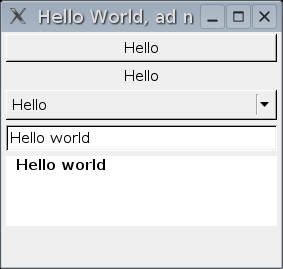
\includegraphics[width=.4\textwidth]{helloWorld}
  \caption{Hello world, how are you?}
  \label{fig:hello-world}
\end{figure}




Well, that will let us make the following simple dialog
(Figure~\ref{fig:hello-world}).


\begin{Scode}
  guitoolkit = new("guiWidgetsToolkittcltk")
  win = gwindow("Hello world", toolkit=guitoolkit)
  label=glabel("Hello world, how are you?", container=win, toolkit=guitoolkit)
  button=gbutton("Close", handler=function(h,...) dispose(win),
  container=win, toolkit=guitoolkit)
\end{Scode}




\end{document}
